\documentclass{article}
\title{Project 2 \\ FYS-STK3155/4155}
\author{Magnus Bergkvam}
\usepackage{url}
\usepackage{amsmath}
\usepackage{graphicx}
\usepackage{subfig}
\usepackage{bm}
\usepackage{listings}

\graphicspath{{../figures/}}


\begin{document}
\maketitle
\bibliographystyle{unsrt}

\section{Abstract}
For the last decade especially, neural networks have been used for more and
more purposes, with them often doing very well in highly complex tasks, with
regression and classification being two of its common applications.
\\

Motivated in exploring these two applications further, we have in this project
tested out how well a basic neural network performs in a regression and a binary
classification example. We then compared this with the linear models we explored
in the previous project \cite{githubrepoproject1} (in the case of regression),
as well as our own implementation of logistic regression (for classification).
For this we have implemented our own neural network code from scratch, where we
have used gradient methods paired with the backpropagation-algorithm.  With
gradient optimization being a central part of the development of both neural
networks and logistic regression we explored ways we can most effectively
optimize the cost function through the Newton-Raphson method, with the various
hyperparameters being central. We also looked at various learning-rate
schedulers, namely Adam, AdaGrad and RMSProp, and also explored with using
regularization for our networks.
\\

What we saw was that in the regression example (using the franke-function we
explored in project 1 \cite{githubrepoproject1}), with regularization, we got some
considerable performance gains compared to the linear models we tested in
project 1, while for classification the neural network did emerge as better, but
with a much finer margin. In the classification result we were able to predict
$100\%$ of the observations in the test-set for our final model, with the
AdaGrad learning-rate scheduler and the sigmoid activation function with two
hidden layers giving us the best fit. Throughout the project we have manifested
the power of neural networks, while simultaneously demystified its components
and the effect that some important hyperparameters have. It comes out that the
learning-rate (and learning-rate scheduler) and regularization parameter are
especially central, while other parameters are less central, but still noticeable.

\section{Introduction}
In the last $10$ or so years, neural networks have really exploded in
popularity. Various different types of neural networks have proved effective for
various different applications all from speech-recognition, to image processing,
to complex language tasks. But how powerful are they really in comparison to
linear models or logistic regression when it comes to basic
regression/classification, and how do we get the most performance out of them?
\\

These are some of the things which we aim to tackle here. To do this we will
implement a rather simple multi-layer perceptron model from scratch using
gradient methods with the backpropagation algorithm for the training. We will
then use our own neural network model for both regression and classification.
For the regression we will be generating data from the franke-function as we did
in project $1$, and of course compare this to the results we got with the linear
models we explored there. For the classification data we will try to classify
whether a patient has cancer or not based on various medical features, where the
wisconsin breastcancer data \cite{breastcancerwisconsin} is the data we will be
using for that.  Additionally we will explore various methods of gradient
optimizations, as both the methods we will implement in this project (i.e.
neural networks and logistic regression) have cost-functions which is typically
minimized w.r.t. its parameters using some sort of gradient method.  As already
mentioned we will implement and explore performances based on various
optimization algorithms, with the ones we will look at in this project being
plain gradient descent, stochastic gradient descent, momentum, AdaGrad, RMSProp
and Adam.  For all our different methods we will compare our own implementations
against established libraries, namely tensorflow and scikit-learn.

There are mainly two reasons why we are specifically focusing on using neural
networks in this project. One is, as already mentioned, that they have become
very popular in the last decade or so, with them being used for more and more
tasks. With their usage increasing it becomes important to understand the way a
model works, and how we get the most amount of performance out of them by
tweaking the various different parts of the network. Additionally since they, in
comparison to a lot of other models, are quite computationally expensive it is
important to realize which of the parameters are the most relevant to tweak, and
which are not so relevant, as this can save a lot of time. Another reason is
because of the universal approximation theorem applying to neural networks. We
will go more deeply into this in \ref{univ-approx-thm}, but the essence is that
a sufficiently big neural network should be able approximate any function
multidimensional function to an arbitrary accuracy
\cite[s.~13.5]{lecutenotes13}. We will see if this property is able to give the
neural networks good results for the regression/classification examples and if
we then are able to outperform models not having this property (linear models /
logistic regression).
\\

We will now get into the methods, before we represent our results, do some
analysis on these results before we conclude. In both the methods and results we
start by look deeper into the pure optimization parts, before going into the
models themselves (i.e. neural networks and logistic regression).

\section{Methods}
\subsection{Basic optimization data}
\label{basicoptdesc}
In part of our analysis we will explore the different parameters for the
different gradient methods. For this we will just use some simple arbitrary data
generated from a fourth order polynomial. The polynomial I have chosen to
generate the data from is:
$$f(x) = 4 - 6 x^2 + x^4.$$
We then just generate a grid of $201$ evenly spaced values $\bm{x}$ on $[-2, 2]$
and generate the response as follows:
$$\bm{y} = f(\bm{x}) + \bm{\epsilon}$$
, where $\epsilon_i \sim N(0, 0.2^2)$, and $f$ is applied element-wise.  We will
use the linear regression and ridge regression for the models, and a
design matrix with fourth-order polynomial features. This way analytical
least-squares solution should give us optimal parameters close to $(4, 0, -6, 0,
      1)^T$. We will mainly explore the effect that the learning-rate and
regularization terms have, and also quickly see the effect of the amount
of epochs and minibatch-size can have. Lastly we will also compare, for a fixed
amount of epochs, which of the optimization methods perform the best, and how
relevant the method of choice is for the final performance.

\subsection{The franke function}
The franke-function is a $2$-dimensional function which we already have explored
in project $1$ \cite{githubrepoproject1}, so I won't go too deeply into this
here. The function is given by:
\begin{align*}
      f(x,y) & = \frac{3}{4}\exp{\left(-\frac{(9x-2)^2}{4} - \frac{(9y-2)^2}{4}\right)}+\frac{3}{4}\exp{\left(-\frac{(9x+1)^2}{49}- \frac{(9y+1)}{10}\right)} \\
             & +\frac{1}{2}\exp{\left(-\frac{(9x-7)^2}{4} - \frac{(9y-3)^2}{4}\right)} -\frac{1}{5}\exp{\left(-(9x-4)^2 - (9y-7)^2\right) }.
\end{align*}
Again we will draw 200 of random observations $\bm{x}_1$ and $\bm{x}_2$, with
$(x_1)_i \in [0, 1]$, and $(x_2)_i \in [0, 1]$ for $1 \leq i \leq 200$. The response will be generated by:
$$\bm{y} = f(\bm{x}_1, \bm{x}_2) + \bm{\epsilon}$$
, with $\epsilon_i \sim N(0, 0.1^2)$ (we apply $f$ element-wise). We will try to
fit a neural network to this data with this time only $\bm{x}_1$ and $\bm{x}_2$
as the response. In project $1$ we added polynomial features of various degrees
to fit to a model. Here we do not need to do this as we can just add enough
nodes and the universal approximation theorem assures us that the network should
do a good job of approximating the function.

\subsection{The wisconsin cancer data}
The wisconsin cancer data \cite{breastcancerwisconsin} is a dataset containing
breast cancer cases, with a response-variable indicating wether the patient has
breast-cancer or not, with some corresponding medical features. This is clearly
a binary classification case, which makes this suitable for both neural networks
and logistic regression models. We will use the dataset included in
\textit{sklearn.datasets} \cite{sklearncancerdata}. To load the data into python
and splitting into train, validation and test sets, we can just use the
following code:

\begin{lstlisting}
X, y = load_breast_cancer(return_X_y=True)
y = y.reshape(len(y), 1)

# Train-test-validation splitting
X_train, X_val, y_train, y_val = train_test_split(X, y, test_size=0.3)
X_val, X_test, y_val, y_test = train_test_split(X_val, y_val, test_size=0.4)
\end{lstlisting}

, after importing \textit{load\_breast\_cancer} from \textit{sklearn.datasets}
\cite{sklearncancerdata} that is.
\\

We split into train, test and validation sets because we will evaluate a lot of
models on the validation set, and then it becomes increasingly important to
evaluate the final selected model on some test set in order for us to not get
too optimistic of a final metric \cite[s.~7.2]{hastie2009elements}.  The data is
limited to $569$ observations with each having $30$ explanatory variables. This
makes both the validation set and test set rather small, so with around $100$
and $70$ observations in each respectively. We then need to be a little
skeptical towards the final metrics, as the metrics may be a little specific to
the split of data.

\subsection{The Newton-Raphson method}
Very central to the numerical optimization we do is the Newton-Raphson method.
This is a method which allows us to find the minimum of some function by using
its gradient. The method has it's origins in the Taylor-expansion of the
function we wish to minimize. In our case we use this to minimize cost-functions
for the models we use. Let $C(\bm{\theta}; \bm{X}, \bm{y})$ be some general
cost-function depending on some design matrix $\bm{X}$ and a response vector
$\bm{y}$. We wish to find the parameter $\bm{\theta}$ which minimizes this cost, given
$\bm{X}$ and $\bm{y}$, i.e. we minimize $C$ with respect to $\bm{\theta}$, while
$\bm{X}$ and $\bm{y}$ are obviously fixed. We can then approximate the cost using a
Taylor-expansion of second order around some value $\bm{\theta}^*$, in which case
we get:
\begin{align*}
      C(\bm{\theta}, \bm{X}, \bm{y}) & \approx C(\bm{\theta}^*; \bm{X}, \bm{y}) + \frac{\partial C(\bm{\theta}^*; \bm{X}, \bm{y})}{\partial \bm{\theta}}(\bm{\theta} - \bm{\theta}^*) + \frac{1}{2} \frac{\partial^2 C(\bm{\theta}; \bm{X}, \bm{y})}{\partial^2 \bm{\theta}}(\bm{\theta} - \bm{\theta}^*)^2 \\
                                     & = C(\bm{\theta}^*; \bm{X}, \bm{y}) + \nabla_{\bm{\theta}} C(\bm{\theta}^*) (\bm{\theta} - \bm{\theta}^*) + \frac{1}{2} \bm{H}_{\bm{\theta}}(\bm{\theta}^*) (\bm{\theta} - \bm{\theta}^*)^2
\end{align*}
Where $\nabla_{\bm{\theta}} C$ is the gradient of $C$ w.r.t. $\bm{\theta}$ and
$\bm{H}_{\bm{\theta}}$ is the Hesse-matrix of $C$ w.r.t.  $\bm{\theta}$. This
should be a good approximation for $C$ sufficiently close to $\bm{\theta}^*$. We
then can find the gradient of this w.r.t. $\bm{\theta}$:
\begin{align*}
      \frac{\partial C(\bm{\theta}, \bm{X}, \bm{y})}{\partial \bm{\theta}} & \approx
      \nabla_{\bm{\theta}} C(\bm{\theta}^*) + \bm{H}_{\bm{\theta}}(\bm{\theta}^*)(\bm{\beta} - \bm{\theta}^*) \\
\end{align*}
If we set this to $0$ to find the minimum we further get:
$$\bm{H}_{\bm{\theta}}(\bm{\theta}^*) (\bm{\theta} - \bm{\theta}^*) = -\nabla_{\bm{\theta}} C(\bm{\theta}^*)$$
which leads to
$$\bm{\theta} - \bm{\theta}^* = - \bm{H}_{\bm{\theta}}(\bm{\theta}^*)^{-1} \nabla_{\bm{\theta}} C(\bm{\theta}^*)$$
and finally
$$\bm{\theta} = \bm{\theta}^* - \bm{H}_{\bm{\theta}}(\bm{\theta}^*)^{-1} \nabla_{\bm{\theta}} C(\bm{\theta}^*)$$

This tells us that the minimum of the Taylor-expansion of the cost-function,
using any $\bm{\theta}^*$ is given as above. The problem with this is that this
is using the Taylor-expansion, which is only reliable close to $\bm{\theta}^*$ so
chances are that using this formula will not give us a global minimum. However
it generally tends to bring us closer to the minimum we are looking after. What
we then usually do is to start with some initial guess for the optimal
$\bm{\theta}$, which we denote $\bm{\theta}^{(0)}$. We then for $k=1, \dots$ let
$\bm{\theta}^{(k)} = \bm{\theta}^{(k-1)} -
      \bm{H}_{\bm{\theta}}(\bm{\theta}^{(k-1)})^{-1} \nabla_{\bm{\theta}}
      C(\bm{\theta}^{(k-1)})$ all the way until we have convergence.

\subsection{Model optimizers and learning-rate schedulers}
Something which often is problematic when using the Newton-Raphson method as
described over is that we need to estimate the Hessian matrix and also invert
it. First of all finding a way to calculate the second derivative can be a
difficulty in and of itself, but it may also be computationally expensive to do
so. Not only that, we also need to invert this matrix which can also become very
computationally expensive, and perhaps also numerically unstable with higher
dimensional hesse matrices (remember that the Hessian matrix is a square matrix
with the same dimensions as $\bm{\theta}$ in both width and height).  Inverting
this matrix then may not be a problem if we only have a few parameters, but for
example when dealing with logistic regression with lots of features, or neural
networks with lots of hidden nodes and layers this becomes unviable. We
therefore will use various methods to approximate this hessian matrix.

\subsubsection{Ordinary gradient descent}
Ordinary gradient descent is a very simple way which we can avoid calculating
this hessian matrix. Here we simply approximate it with some numerical
learning-rate, which we will throughout this report denote $\eta$. This way our
algorithm becomes:
$$\bm{\theta}^{(k)} = \bm{\theta}^{(k-1)} - \eta \nabla_{\bm{\theta}} C(\bm{\theta}^{(k-1)}).$$
Often we may just keep $\eta$  fixed throughout all the iterations, but we can
also make it depend on $k$. For example one may wish to start with a higher
learning-rate and make this decrease with the number of iterations. This method
I will refer to as using time-decay.  When using gradient descent for training
our model, $\eta$ then becomes a hyperparameter in this model. Often this
hyperparameter is rather important in determining the fit of the model. We often
want a rather high learning-rate as this will lead to faster convergence towards
some optimum, however if we make it too big we may not get convergence at all. I
will mainly throughout the code simply set up a grid of learning-rates and fit
to all of them, and simply choose the learning-rate which gives the best
performance for some fixed amount of epochs, but there also exists other more
advanced ways of tuning this parameter.

\subsubsection{Stochastic gradient descent}
Stochastic gradient descent is very similar to ordinary gradient descent, except
the fact that instead of training for each epoch on the whole dataset we split
the data into $n$ randomly chosen mini-batches each of some specified size (this
is what \textit{minibatch\_size} in our code and report will refer to). Then we
do training over all of the $n$ mini-batches for each epoch, while the rest of
the method remains the same.

\subsubsection{Momentum}
One problem with gradient descent and stochastic gradient descent which one
often can see is that it can be quite slow to learn. Ideally we would like the
model to minimize the cost/loss as quickly as possible, and therefore one might
want to use methods designed to accelerate this learning process. One relatively
simple such method is using a momentum, which often accelerates learning quite
drastically especially in cases with high curvatures and small consistent or
noisy gradients \cite[s.~8.3.2]{goodfellow2016deep}. This method introduces a
variable $\bm{v}$ which describes the direction and speed which the parameter
$\bm{\theta}$ is moving in parameter space \cite[s.~8.3.2]{goodfellow2016deep}, much
like the role of velocity in physics. To calculate this $\bm{v}$ we need a
hyperparameter $\alpha \in [0, 1)$ (we will use $\alpha = 0.9$ throughout this
project) and we initialize $\bm{v} = \bm{0}$. Then for each learning-iteration
we update $\bm{v}$ the following way:
$$\bm{v} = \alpha \bm{v}_{prev} - \eta \Delta_{\bm{\theta}} C(\bm{x}, \bm{y}, \bm{\theta}).$$
We then can simply update the $\bm{\theta}$ as follows:
$$\bm{\theta} = \bm{\theta}_{prev} + \bm{v}$$
We then see that the value of the $\bm{v}$ will depend on the current cost-gradient
w.r.t. $\bm{\theta}$ as well as the previous $\bm{v}$, which again depends on
the previous cost-gradient w.r.t. $\bm{\theta}$ and the previous previous
$\bm{v}$ and so on. Therefore we see that $\bm{v}$ is influenced by all the
previous cost-gradients, weighted differently, in contrast to just using the
current cost-gradient, and granted they point in a somewhat similar direction,
the $\bm{v}$ will grow bigger and bigger in size. It is therefore not that
difficult to see that this can give quicker learning.


Keep in mind that in theory there is nothing stopping us from combining momentum
with any of the other methods we discuss here, however methods like Adam already
incorporates a form of momentum \cite[s.~8.5.3]{goodfellow2016deep}, so we might
not get much quicker learning by using it, if any at all.

\subsubsection{AdaGrad}
\label{adagradsec}
AdaGrad is another way designed to give faster learning. This is an algorithm
which uses adaptive learning-rates. These have a difference in that each axis of
the parameter-space $\bm{\theta}$ essentially get a separate learning-rate
\cite[s.~8.5]{goodfellow2016deep}, while these separate learning-rates change/adapt
throughout the learning process, which is a different approach to using momentum.
AdaGrad is a rather simple way of achieving a good such adaptive learning-rate.
It scales down the parameters with big historical updates, and scales up the
ones with small corresponding historical updates up
\cite[s.~8.5.1]{goodfellow2016deep}.  For AdaGrad we introduce one variable
$\bm{r}$ which we initially set to $\bm{0}$, as well as a small constant
$\delta$ which we typically set to $10^{-7}$. The algorithms is as follows until
the stopping-criterion is met \cite[algorithm~8.4]{goodfellow2016deep}:
\begin{itemize}
      \item Sample a minibatch of $m$ observations from the training-set
            consisting of $\{\bm{x}^{(1)}, \dots, \bm{x}^{(m)}\}$ as the explanatory
            variables and $\{\bm{y}^{(1)}, \dots, \bm{y}^{m}\}$.
      \item Calculate the gradient $\bm{g}$ of the cost w.r.t. $\bm{\theta}$ using
            this minibatch.
      \item Update the $\bm{r}$ to become $\bm{r}_{prev} + \bm{g} \odot \bm{g}$
            ($\odot$ being the Hadamard-product).
      \item Calculate $\Delta \bm{\theta} = -\eta
                  \frac{1}{\delta + \sqrt{\bm{r}}} \odot \bm{g}$ and update
            $\bm{\theta}$ accordingly (i.e. set $\bm{\theta} =
                  \bm{\theta}_{prev} + \Delta \bm{\theta}$).

\end{itemize}

\subsubsection{RMSProp}
RMSProp is much like AdaGrad, but is designed to be more robust for
non-convex cost-function settings \cite[s.~8.5.2]{goodfellow2016deep}, like
typical neural nets. Unlike AdaGrad where we shrink the learning-rates using the
sizes of all the previous updates, RMSProp focuses less on the history of
updates from very long ago, but otherwise using much of the same approach. The
RMSProp algorithm requires therefore a decay-rate $\rho$ as a hyperparameter as
well, along the $\bm{r}$ which we again initialize to be $\bm{0}$. Here we also need a
small constant $\delta$, which typically is set to $10^{-6}$. Then we do the
following until the stopping-criterion is met \cite[algorithm~8.5]{goodfellow2016deep}:
\begin{itemize}
      \item Sample a minibatch of $m$ observations from the training-set
            consisting of $\{\bm{x}^{(1)}, \dots, \bm{x}^{(m)}\}$ as the explanatory
            variables and $\{\bm{y}^{(1)}, \dots, \bm{y}^{m}\}$.
      \item Calculate the gradient $\bm{g}$ of the cost w.r.t. $\bm{\theta}$ using
            this minibatch.
      \item Update the $\bm{r}$ to become $\rho \bm{r}_{prev} + (1 - \rho) \bm{g} \odot \bm{g}$
            ($\odot$ being the Hadamard-product)
      \item Calculate $\Delta \bm{\theta} = -\eta \frac{1}{\sqrt{\delta + \bm{r}}}
                  \odot \bm{g}$ and update $\bm{\theta}$ accordingly (i.e. set $\bm{\theta} =
                  \bm{\theta}_{prev} + \Delta \bm{\theta}$).
\end{itemize}

\subsubsection{Adam}
Adam is a very popular learning-rate scheduler, and it is probably the method we
will tackle here which most often gives the best results.
\cite[s.~8.6.1]{goodfellow2016deep}. We start the algorithm by initializing the
parameter $\bm{\theta}$ which we would like to optimize the cost/loss w.r.t.
(typically we initialize this by drawing it randomly from for example the normal
distribution which is what we have done in this project). We also set beforehand
$\bm{s} = \bm{0}$, $\bm{r} = \bm{0}$ and $t=0$. Here the algorithms is as
follows until we meet the stopping criterion \cite[algortihm~8.7]{goodfellow2016deep}:
\begin{itemize}
      \item Sample a minibatch of $m$ observations from the training-set
            consisting of $\{\bm{x}^{(1)}, \dots, \bm{x}^{(m)}\}$ as the explanatory
            variables and $\{\bm{y}^{(1)}, \dots, \bm{y}^{m}\}$.
      \item Calculate the gradient $\bm{g}$ of the cost w.r.t. $\bm{\theta}$ using
            this minibatch.
      \item Increment $t$ by $1$ (i.e. set $t=t_{prev}+1$).
      \item Update $\bm{s}$ to become $\rho_1 \bm{s}_{prev} + (1 - \rho_1)\bm{g}$.
      \item Update $\bm{r}$ to become $\rho_2 \bm{r}_{prev} + (1 - \rho_2)g \odot
                  g$ ($\odot$ again being the Hadamard-product).
      \item Correct the bias in the first moment by: $\hat{\bm{s}} = \frac{\bm{s}}{1 - \rho_1^t}$.
      \item Correct the bias in the second moment by: $\hat{\bm{r}} = \frac{\bm{r}}{1 - \rho_2^t}$.
      \item Finally calculate $\Delta \bm{\theta} = -\eta
                  \frac{\hat{\bm{s}}}{\sqrt{\hat{\bm{r}}} + \delta}$ and update $\bm{\theta}$
            accordingly (i.e. set $\bm{\theta} = \bm{\theta}_{prev} + \Delta
                  \bm{\theta}$).
\end{itemize}
Here $\eta$ is referred to as the step-size (but we will use the term
learning-rate instead), $\rho_1$ and $\rho_2$ are the decay-rate which must be
in $[0, 1)$ (typically we set the defaults to $\rho_1 = 0.9$ and $\rho_2 =
      0.999$), $\delta$ is just a small constant (we set it to $10^{-8}$). Note that
we for all these three adaptive methods we can in theory just drop the minibatch
sampling and still get a functioning algorithm, but this will often give worse
results.

\subsubsection{Object-oriented code for the learning-rate schedulers}
Being one of the most central parts of the project, we have chosen to implement
the learning-rate schedulers as an abstract base class in python. The abstract
base class is implemented as follows:

\begin{lstlisting}
class Scheduler(abc.ABC):
    def __init__(
        self,
        learning_rate: float,
        timedecay: typing.Callable[[int], float] = lambda _: 1,
        use_momentum=False,
        momentum_alpha=0.9,
    ):
        self._learning_rate = learning_rate
        self._momentum_alpha = momentum_alpha
        self._timedecay = timedecay
        self._update: np.ndarray | None = None
        self._use_momentum = use_momentum
        self.reset()

    @property
    def learning_rate(self):
        return self._learning_rate * self._timedecay(self._current_epoch)

    @abc.abstractmethod
    def _update_no_momentum(self, grad):
        pass

    def update(self, grad) -> np.ndarray:
        self._current_epoch += 1
        if self._use_momentum:
            if self._update is None:
                self._update = np.zeros_like(grad)

            self._update = self._update_no_momentum(grad) + self.momentum()
        else:
            self._update = self._update_no_momentum(grad)

        return self._update

    def momentum(self):
        return self._momentum_alpha * self._update

    def reset(self):
        self._current_epoch = 0
\end{lstlisting}

This way to add support for more schedulers we can just implement a separate
class for the scheduler with the algorithm implemented by overriding
\textit{\_update\_no\_momentum}, and overriding other methods as necessary, and
it should work well with the rest of our code.

\subsection{Automatic differentiation}
What is clear is that in our optimization it will be central to calculate the
gradient of some loss function with respect to some parameter, however it is not
always easy to find analytical gradients by hand. Automatic differentiation is
an algorithmic approach to calculating the gradients of functions. We will take
some usage of this in our code through the python-library jax
\cite{githubrepojax}, but this is a somewhat minor part of the project so I
won't go too much into detail about how this algorithm works in detail. Broadly
said, automatic differentiation utilizes clever applications of the chain rule
in order to calculate the gradients of functions without compromising on
accuracy (it usually gives almost exactly the same results as an analytical
expression).  We will utilize this in some of our optimizations instead of
calculating gradients by hand, and for adding support in our code so that users
don't have to manually calculate gradients by hand, which can be time-consuming,
and a potential for errors in the calculations. The reason we have not used it
throughout all the codes is mainly due to the fact that using automatic
differentiation often makes our code considerably more computationally
expensive, and a lot of our programs are already computationally expensive
enough.

\subsection{Neural networks}
There are many different implementations of neural networks out there. We will
in this project focus on one of the simplest ones to implement, namely the
multi-layer-perceptron. The multi-layer perceptron consists of a input layer
with $p$ nodes (granted we have $p$ covariates), as many hidden layers as we
want, each of which can have also as many nodes as we want, and then an output
layer of the same dimensionality as our response. For our notation in this
section we will assume we have $L$ total layers (excluding the input layer), or
equivalently $L-1$ hidden layers. Linking the layers together is a set of
weights, where each node in the layer before is connected to each node in the
next layer. Additionally each layer has its own weight matrix $\bm{W}^{(l)}$ and bias
vector $\bm{b}^{(l)}$ for $1 \leq l \leq L$. Each layer also has its own
activation function, which we denote $f^{(l)}$, again for $1 \leq l \leq
      L$. Typical choices of activation functions are sigmoid, relu or leaky relu,
which are the ones we will explore in this project. For the final layer we
instead call this the output function. The output function is typically tailored
to whichever data we have. If we for example want to do regression we often just
set this to the identity-function, i.e. we do not transform the activations at
all. This is largely due to the fact that we then typically need an unbounded
and continuous function when doing regression, and for most cases the identity
function does the job well, while also being very simple. In the case where we
are doing classification we this choice is no longer a good one as the identity
function is not bounded, and we in that case want the output to be a probability
between $0$ and $1$, so then a sigmoid-function for example is a good choice.
Predictions are made using forward propagation (this algorithm we describe in
\ref{forwardprop}), calculating the next layer activations based on the layer
activation in the layer before, until we are at the final layer. Here we will
follow the notation of \textit{Deep Learning}\cite{goodfellow2016deep} by
denoting $\bm{a}^{(l)}$ as the activations in layer $l$ before applying the
activation functions and $\bm{h}^{(l)}$ as the final activations in layer $l$
(i.e. after applying the activation function).  Keep in mind that the final
predictions then will be $\bm{h}^{(L)}$, while the activations in the inputs
(which is just the values of the features) are denoted $\bm{h}^{(0)}$. For
fitting the networks we use the backpropagation algorithm, where we for some
given some design matrix $\bm{X}$ we fit $\hat{\bm{y}} = \bm{h}^{(L)}$ to match
some target output $\bm{y}$ for a given cost-function $C(\hat{\bm{y}}, \bm{y})$
as good as possible.

\subsubsection{Regularization}
We will also implement basic support for regularization. This requires a
regularization function $\Omega(\bm{\theta})$, where $\bm{\theta}$ in this case
corresponds to all the parameters. Additionally we add a regularization parameter
$\lambda$ which scales the extent of regularization we apply. Here we will only
add $l_2$ regularization, so $\Omega(\bm{\theta}) = \frac{1}{2}\bm{\theta}^T
      \bm{\theta}$. How the regularization is used we will go into mainly in
\ref{backprop}, but we will also need the gradient of this regularizer with
respect to the weights in each layer. For the $l_2$ regularization, we see that we have:
$$\Omega(\bm{\theta}) = \frac{1}{2} \left( \sum_{l = 1}^{L} \sum_{i = 1}^{n_{i-1}} \sum_{j = 1}^{n_i} {\bm{W}_{i j}^{(l)}}^2 + \sum_{l = 1}^{L} {\bm{b}^{(l)}}^T \bm{b} \right)$$.
Taking the derivative with respect to $\bm{W}_{i j}^{(l)}$ we get:
\begin{align*}
      \frac{\partial \Omega(\bm{\theta})}{\partial \bm{W}_{i j}}^{(l)} & = \frac{1}{2} \frac{\partial {\bm{W}_{i j}^{(l)}}^2}{\partial \bm{W}_{i j}^{(l)}} \\
                                                                       & = \bm{W}_{i j}^{(l)}
\end{align*}
Hence we get that $\nabla_{\bm{W}^{(l)}} \Omega(\bm{\theta}) = \bm{W}^{(l)}$.\\
Keep in mind that we do not include regularization on biases.  This is because
we usually are ok with having sizeable values for the biases, more so that we
are with having big values for weights, which often results in high degree of
overfitting. Seeing as there are a lot more weights than biases, more model
complexity is also reduced by penalizing the weights than the biases.

\subsubsection{Forward propagation algorithm}
\label{forwardprop}
With the description of the model out of the way, the forward propagation is actually
rather simple. We assume we have $L-1$ hidden layers, with index $L$ being the
output layer. We let us inspire by algorithm 6.3 in \textit{Deep Learning}
\cite[p.~212]{goodfellow2016deep}, with some practical improvements for the
code. Our algorithm becomes:
\begin{itemize}
      \item Set $\bm{h}^{(0)} = \bm{X}$
      \item \textbf{for} $l = 1, \dots, L$ \textbf{do}
      \item $\bm{a}^{(l)} = \bm{h}^{(l-1)} \bm{W}^{(l)} + \bm{b}^{(l)}$ (here $\bm{b}^{(l)}$ is added for every row).
      \item $\bm{h}^{(l)} = f^{(l)}(\bm{a}^{(l)})$ (here we apply $f$ element-wise)
      \item \textbf{end for}
      \item $\hat{\bm{y}} = \bm{h}^{(L)}$
\end{itemize}
Keep in mind that here that $\bm{X}$, $\bm{y}$, $\bm{a}$-s, $\bm{h}$-s are
allowed to be matrices. Here if $\bm{X}$ is a $n \times p$ matrix, it is easy to
see that $\bm{a}^{(l)}$ and $\bm{h}^{(l)}$ are going to be $n \times n_l$
matrices ($n_l$ being the amount of nodes in hidden layer $l$), i.e. we have
that each row represents the activations in layer $l$ for each observation. Then
as a consequence since $\hat{\bm{y}} = \bm{h}^{(L)}$, we have that each row in
the prediction matrix corresponds perfectly to the prediction of each row of the
design/feature matrix.

\subsubsection{Backward propagation algorithm}
\label{backprop}
The backward propagation algorithm is a way for us to calculate the gradients of
the weight and biases matrices/vectors. isn't all that much more complicated.
Again we take big inspiration from \textit{Deep Learning}, this time algorithm
6.4, with some tweaks. The backwards propagation algorithm then goes as follows:
\begin{itemize}
      \item Set $\bm{g} = \nabla_{\hat{\bm{y}}} C(\hat{\bm{y}}, \bm{y})$
      \item \textbf{for} $l = L, \dots, 1$ \textbf{do}
      \item Update $\bm{g}$ by setting $\bm{g} = \bm{g} \odot {f^{(l)}}' (\bm{a}^{(l)})$
      \item Calculate $\nabla_{\bm{b}^{(l)}} L(\hat{\bm{y}}, \bm{y}) = \sum_{i=1}^n \bm{g}_{i *}$ (sum over all the rows)
      \item Calculate $\nabla_{\bm{W}^{(l)}} L(\hat{\bm{y}}, \bm{y}) = {\bm{h}^{(l)}}^T \bm{g} + \lambda \nabla_{\bm{W}^{(l)}} \Omega(\bm{\theta})$
      \item \textbf{end for}
\end{itemize}
Then having gathered the gradients of the weights/biases from this we can then
use whichever gradient-method we please to update the weights/biases, and
continue this way until we have convergence (or the max amount of epochs is
reached).

\subsubsection{Weight and bias initialization}
We see that at the core of neural networks are the weight-matrices and bias
vectors, and seeing as we want to use an iterative method (namely the
Newton-Raphson method) it becomes clear that we need to initialize the weights
and biases to something. If we were to initialize all the weights/biases to be
$0$ (or some other constant) all of the neurons in the hidden layers will all
have the same activations in the first iteration, and it becomes impossible for
the model to learn properly. Our solution to this is to draw the weights randomly, for
example from the standard-normal distribution as we have done in this project.
This way we will be able to tackle the problem of the learning-process not
starting properly. Another thing to take into consideration is that we ususally
want the weights to be quite small initially, as very big weights can lead to
overfitted models. For biases we often don't always bother initializing these
randomly (although there is nothing hindering us to do so).  What we will do is to
initialize all the biases to the same value in every layer (we will set all of them to
$0.1$).  Setting it to a small positive value will ensure that all the neurons
are activated in the first training-cycle, which will also ensure all the
neurons have some output which will be backpropagated in the first
training-cycle \cite[s.~Weights and biases]{week41}.

\subsubsection{The universal approximation theorem}
\label{univ-approx-thm}
The universal approximation theorem tells us that if we have a neural network
with one hidden layer and a non-linear activation-function in the hidden layer,
if we have enough nodes in the hidden layer we should be able to approximate any
continous multi-dimensional function to any accuracy
\cite[s.~13.5]{lecutenotes13}. Keep in mind that this is merely to the
training-data. A neural network can be able to approximate the training-data
very well, without necessarily getting that great performance for new data.

\subsection{Activation functions}
For this project we will explore three different activation functions for the
hidden layers.
\subsubsection{Sigmoid}
The sigmoid activation function limits the activations of the neurons between
$0$ and $1$. The sigmoid activation function is given as the following:
$$\sigma(x) = \frac{1}{1 + \exp(-x)}$$
With the derivative being (this is quite straightforward to calculate):
$$\sigma'(x) = \sigma(x) (1 - \sigma(x))$$
Additionally as mentioned this will also be used as an output-function when we
are doing binary classification, due to the fact that the final neuron
activations will be between $0$ and $1$.

\subsubsection{Relu}
\label{relu-desc}
Another popular activation function we will use is the relu activation function.
Unlike the sigmoid function this does not have a upper bound. The function then
can be expressed by:
$$\text{relu}(x) = \max(x, 0)$$
The derivative then becomes:
$$\text{relu}'(x) = \begin{cases}
            0 \qquad & \text{if } x < 0 \\
            1        & \text{if } x > 0
      \end{cases}$$
Keep in mind that the derivative is not defined for $x=0$. This however is
usually unproblematic as we almost never get activations being exactly $0$. In
our implementation we will just set the derivative to $0$ if the activation is
exactly $0$ (but again this should more or less never happen).

\subsubsection{Leaky relu}
The leaky relu is a generalization of the relu-function which unlike the
relu-function doesn't completely neutralize negative values.  Technically this
makes this function not bounded below, however with $\delta$ being rather small
severely limits the size of the negative activations, while no such shrinkage is
applied for the positive activations of course. The leaky relu is given by:
$$\text{lrelu}(x) = \begin{cases}
            x \qquad & \text{if } x > 0    \\
            \delta x & \text{if } x \leq 0
      \end{cases}$$
The derivative then becomes:
$$\text{lrelu}'(x) = \begin{cases}
            \delta \qquad & \text{if } x < 0 \\
            1             & \text{if } x > 0
      \end{cases}$$
We see one major difference between this and the relu is that for negative
activations, the derivative of this will not be $0$, but $\delta$. This means
that the network will be able to learn on activations which are negative as
well, albeit likely slower than the positive cases. For this project we will be
using $\delta = 10^{-3}$.

\subsection{Cost functions}
In this project we will use mainly two activation functions, namely mse/sse for
regression and cross-entropy for binary-classification. We will now quickly go
into these.

\subsubsection{MSE/SSE}
A natural choice of cost-function when dealing with regression tasks is the MSE.
When the target dimensions are always $1$ (which they are in this project), the
MSE is defined like:
$$\text{mse}(\hat{\bm{y}}, \bm{y}) = \frac{1}{n} \sum_{i=1}^n (\hat{\bm{y}}_i - \bm{y}_i)^2 = \frac{1}{n}(\hat{\bm{y}} - \bm{y})^T (\hat{\bm{y}} - \bm{y})$$
The derivative with respect to $\hat{\bm{y}}$ then becomes:
$$\frac{\partial \text{mse}}{\partial \hat{\bm{y}}}(\hat{\bm{y}}, \bm{y}) = \frac{2}{n} (\hat{\bm{y}} - \bm{y})$$
We will also use the total sum of squares (SSE). Minimizing this is the same as
minimizing the MSE, but with one less floating-point operation. The SSE is given
by:
$$\text{sse}(\hat{\bm{y}}, \bm{y}) = \sum_{i=1}^n (\hat{\bm{y}}_i - \bm{y}_i)^2 = (\hat{\bm{y}} - \bm{y})^T (\hat{\bm{y}} - \bm{y})$$
and its derivative then becomes:
$$\frac{\partial \text{sse}}{\partial \hat{\bm{y}}}(\hat{\bm{y}}, \bm{y}) = 2(\hat{\bm{y}} - \bm{y})$$
The only potential problem with using SSE instead of MSE is that the gradient
will then be dependent on the amount of observations we are using, which can be
problematic with stochastic gradient descent. However in this project we will
set a fixed size of each minibatch, which guarantees that each training-set sent
into this cost/loss function will be of the same size, so this becomes
unproblematic.

\subsubsection{Cross-entropy}
For binary classification we will use cross-entropy as out cost-function.
Minimizing the cross-entropy is equivalent to maximizing the likelihood. We have
the cross-validation given by:
$$\text{cross-entropy}(\hat{\bm{y}}, \bm{y}) = -\sum_{i=1}^{n} ( \bm{y}_{i} \log(\hat{\bm{y}}_i) + (1 - \bm{y}) \log(1 - \hat{\bm{y}}_i) ).$$
With the gradient w.r.t. $\hat{\bm{y}}$ then becoming:
$$\frac{\partial \text{cross-entropy}}{\partial \hat{\bm{y}}}(\hat{\bm{y}}, \bm{y}) = (\hat{\bm{y}} - \bm{y}) / ((1 - \hat{\bm{y}}) \odot \hat{\bm{y}}).$$
Here the division is element-wise. One thing to note is that we see that if one of
our predictions $\hat{\bm{y}}_i$ is very close to $0$ while the target value is $1$
or vice versa, which especially can happen in the first iterations when using
some sort of unbounded activation function in the last hidden layer, the
gradient can become very big. If we get too big of a gradient this can be
problematic for many reasons, with one being we can get values too big for the
computer to calculate. In our code we will solve this by clipping the
predictions in the cross-entropy-gradient, so that they don't become too close
to $0$ or $1$ so that this doesn't become a problem. Additionally we will add a
small $\delta$ inside the log-expression in the cross-entropy function for the
same reason.

\subsection{Accuracy score}
For classification methods, after we have fitted the models and made predictions,
we often want to evaluate a metric of how good our model really is. One intuitive
such metric we will use a lot is the accuracy score. The accuracy-score
essentially is just the proportions of datapoints we have classified correctly
on some data. The accuracy score can then be defined as follows:
$$\frac{1}{n} \sum_{i=1}^n I(\hat{\bm{y}}_i = \bm{y}_i).$$
Using numpy this can simply be written as:
\begin{lstlisting}
np.mean(y_pred == y)
\end{lstlisting}
, for some predictions \textit{y\_pred} and some target \textit{y}. Keep in mind
that while this can tell us the overall successes/failures of classifications it
does not tell us what kinds of prediction errors we have made. For example in a
binary-classification problem we may be interested in finding the amount of
predictions we have made to be $1$ while the target was $0$, or vice versa, as
one of these predictions errors may be more severe than the other. For these
cases we have a confusion-matrix plotting the predictions against the target in
a heatmap. We will use some such plots in this project as well.

\subsection{Model complexities}
One final thing to consider which will be very important for our results is the
model-complexity of neural networks and logistic regression. Logistic regression
requires just as many parameters as we have explanatory variables, so the model
complexity is rather low, at least in the case where we don't have too many
covariates. Neural networks however contain a lot of parameters so naturally the
model is also much more complex. In both cases however we can introduce
regularization constraints, so we are able to control the model complexities in
both cases.

\subsection{Logistic regression}
The logistic regression model is a commonly used, and rather simple, way to
perform classification tasks. With logistic regression we assume a binary
response $0$ and $1$ typically and model the probability the follwing way:
$$Pr(Y_i = 1 | \bm{x}_i) = \frac{1}{1 + \exp(\bm{x}_i \bm{\beta})} = \sigma(\bm{x}_i \bm{\beta})$$
, where $\sigma$ is obviously the sigmoid-function as already described. We then
can do classification based on this, where we typically classify to $1$ if this
probability is bigger than $0.5$ (this is the boundary we will use here) and $0$
if lower than $0.5$. In order to estimate the $\bm{\beta}$ parameters we use the
likelihood for such a model, given by \cite[s.~4.4]{hastie2009elements}:
$$l(\bm{\beta}) = \sum_{i=1}^{n} (y_i \bm{x}_i \bm{\beta} - \log(1 + \exp(\bm{x}_i \bm{\beta})))$$
, where the estimates $\hat{\bm{\beta}}$ become the ones which maximize this
likelihood. The cost-function then becomes:
$$C(\bm{\beta}) = -\sum_{i=1}^{n} (y_i \bm{x}_i \bm{\beta} - \log(1 + \exp(\bm{x}_i \bm{\beta}))).$$
To minimize we need the gradient given by \cite[s.~4.4]{hastie2009elements}:
$$\frac{\partial C(\bm{\beta})}{\partial \bm{\beta}} = -\sum_{i=1}^{n}\bm{x}_i^T(y_i - Pr(Y_i = 1 | \bm{x}_i)) = -\bm{X}^T(\bm{y} - \bm{p}).$$
We then can use the Newton-Raphson method on this in order to estimate the $\bm{\beta}$.
\\

We may also want to add regularization. To do this we can simply add a term
$\frac{1}{2}\lambda \bm{\beta}^T \bm{\beta}$ to the cost-function, and add a term
$\lambda \bm{\beta}$ to its gradient, just as we did with neural networks.

\section{Results}

\subsection{General optimization}
The \textbf{optimization\_basic.py} in the project repo
\cite{githubrepoproject2code} performs various experimentation on some generated
data as described in \ref{basicoptdesc}, and explores the effects the
various parameters have when using gradient methods. For exploring the effect
the amount of epochs has, we did a quick test by four-doubling the amount of
epochs from one model to another. Table \ref{epochs-varying} shows the results
of optimizing using GD and SGD with different amount of epochs. What we clearly
see is that in general the more amount of epochs we allow the smaller the cost
will be (granted we have convergence for the specified learning-rate). This is intuitive
as for each iteration we should get closer to the minimum of the cost, so doing
more iterations must also naturally bring us closer to the minimum.

\begin{table}
      \centering
      \begin{tabular}{| c | c | c |}
            Epochs   & 100  & 400  \\
            COST GD  & 4.51 & 1.56 \\
            COST SGD & 0.13 & 0.04
      \end{tabular}
      \caption{The cost (mean-squared-error) of the model for plain gradient
            descent and stochastic gradient descent, trained with $100$ epochs and
            $400$ epochs. In both cases the model trained on more epochs is
            substantially smaller.}
      \label{epochs-varying}
\end{table}

For stochastic gradient descent we may also be interested in seeing if the size
of the minibatches has an effect on the speed we are able to learn. Table
\ref{minibatchsize-varying} shows the effect at which the minibatch-size
influences how quick we are able to minimize the cost. Here we see that the
lower minibatch-sizes seem to give a little quicker learning, but that  this
effect is not that enormous (perhaps with the exception of the difference
between the minibatch-sizes of $8$ and $32$, where there is quite a difference).

\begin{table}
      \centering
      \begin{tabular}{| c | c | c | c | c |}
            Minibatch-size  & 8      & 12     & 16     & 32     \\
            COST SGD (best) & 0.0421 & 0.0612 & 0.1315 & 0.7856
      \end{tabular}
      \caption{The cost (mean-squared-error) of the model for stochastic
            gradient descent trained on a grad of learning-rates for each
            minibatch-size with the learning-rate giving the lowest cost is chosen. We
            see that in this case the lower minibatch-sizes seem give faster
            learning. Here we have trained using $100$ epochs.}
      \label{minibatchsize-varying}
\end{table}

We also trained the various methods using stochastic gradient descent on some
learning-rate grid. The costs of these functions plotted against the
learning-rates at which the cost was obtained is shown in figure
\ref{learningrate-cost-plot}. We see that generally that the bigger the
learning-rate is the better it is, however we also see that if it gets too high
then we get that the cost diverges towards infinity. We also can see that in all
the cases the learning-rate is very important, with higher learning-rates giving
much quicker learning.

Just from this plot we see quite a big difference between how quick the
different optimization-methods work, with the momentum versions being much
quicker to minimize the costs. Table \ref{gradmethods-comparison} shows the
costs for the different methods of calculating the learning-rates. We see that
in all cases adding momentum increases the speed of learning by quite a bit
(perhaps less so with AdaGrad trained on stochastic minibatches, where this
increase is quite marginal). We see that which method we use does impact the
speed of learning by quite a lot, with the lowest cost (stochastic AdaGrad with
momentum) being more than $100$ times smaller than the highest cost (GD without
momentum). Overall we can see that AdaGrad did seem to perform the best out of
the methods we tried out.

We also check out the performance of each method under a different
cost-function, namely using a ridge cost-function. Previously we have explored
how the performance depends on the hyperparameters isolated. In ridge regression
we introduce another hyperparameter, namely the regularization parameter
$\lambda$. Since we are dealing with ridge regression here it makes sense to
explore the mse on some test-data, which is what we have done in the program.
This now doesn't only depend on the learning-rate $\eta$ anymore as previously,
but also the regularization parameter $\lambda$ (we keep the rest of the
parameters fixed).  Figure \ref{heatmapplot-lr-lambda-gd-sgd} shows a heatmap
which tells us how this depends on both the $\eta$ and $\lambda$ for GD and SGD.
What we see is that the best performance is quite sensetive to both the $\eta$
and $\lambda$, and that a wrong $\eta$ or $\lambda$ alone can very much ruin the
performance. Similarly figure \ref{heatmapplot-lr-lambda-adagrad} shows a corresponding
plot for AdaGrad. Here we see that this is much more robust to higher
learning-rates than the other methods, where it seems to take much more for this
to diverge. This is probably related to the fact that AdaGrad vastly downscales
the learning in directions with high historical updates (see \ref{adagradsec})
so this is able to combat divergence for the cost for the higher learning-rates.

For both the figure \ref{heatmapplot-lr-lambda-gd-sgd} and
\ref{heatmapplot-lr-lambda-adagrad}, focusing on the regularization parameter
$\lambda$ we see much of the same as we did with normal ridge, where a too low
$\lambda$ did not give that good results because of too little regularization,
while a too high $\lambda$ also caused subpar results due to too much
regularization. However, we also see that we now have another dimension on top
determining the performance, namely that the learning-rate must also be optimal
for the model to be any good. Picking too low of a learning-rate will as seen
already cause the cost to not converge, while picking a too big learning-rate
will cause the cost to diverge. Picking a good model clearly requires us to do some
kind of hyperparameter-tuning (like a grid-search for example) on both $\eta$
and $\lambda$, as some $\eta$-values will cause a diverging cost for some, but
not all, values of $\lambda$ (as can be seen for $\eta = 1$ for the SGD case in
figure \ref{heatmapplot-lr-lambda-gd-sgd}).

\begin{figure}
      \centering
      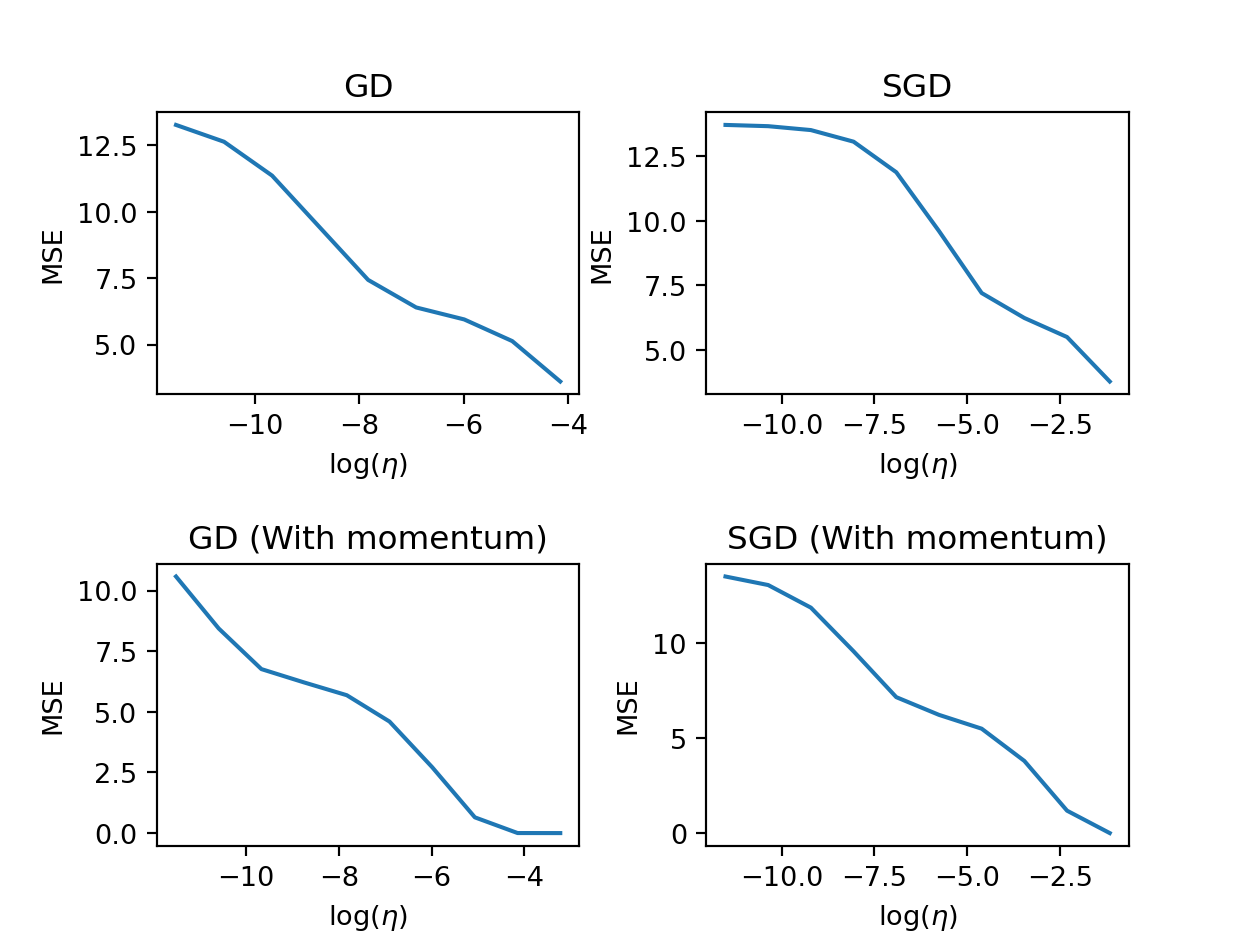
\includegraphics[scale=0.8]{optimizers_plot}
      \caption{The costs trained on specific learning-rates. We see a general
            downward-moving trend, until we get a learning-rate higher than
            $\sqrt{10}$ for the SGD cases, and $10^{-2}$, and
            $10^{-\frac{3}{2}}$ for the GD cases without and with momentum
            respectively, in which case after this we get a diverging cost.}
      \label{learningrate-cost-plot}
\end{figure}

\begin{table}
      \centering
      \begin{tabular}{| c | c | c | c | c |}
            Method name          & GD     & SGD    & AdaGrad (non-sgd) & AdaGrad (sgd) \\
            COST (no momentum)   & 4.5150 & 4.1092 & 1.4655            & 0.0418        \\
            COST (with momentum) & 0.0384 & 0.0488 & 0.0400            & 0.0385
      \end{tabular}
      \caption{Various different learning-rate scheduling methods, with the
            methods being trained for a grid of learning-rates $\eta$, with the best
            cost being selected. Here for the stochastic gradient descent, we
            have used a timedecay for the learning-rate (plain gradient descent
            only). AdaGrad (sgd) here refers to using AdaGrad and training on
            stochastic mini-batches.}
      \label{gradmethods-comparison}
\end{table}

\begin{figure}
      \centering
      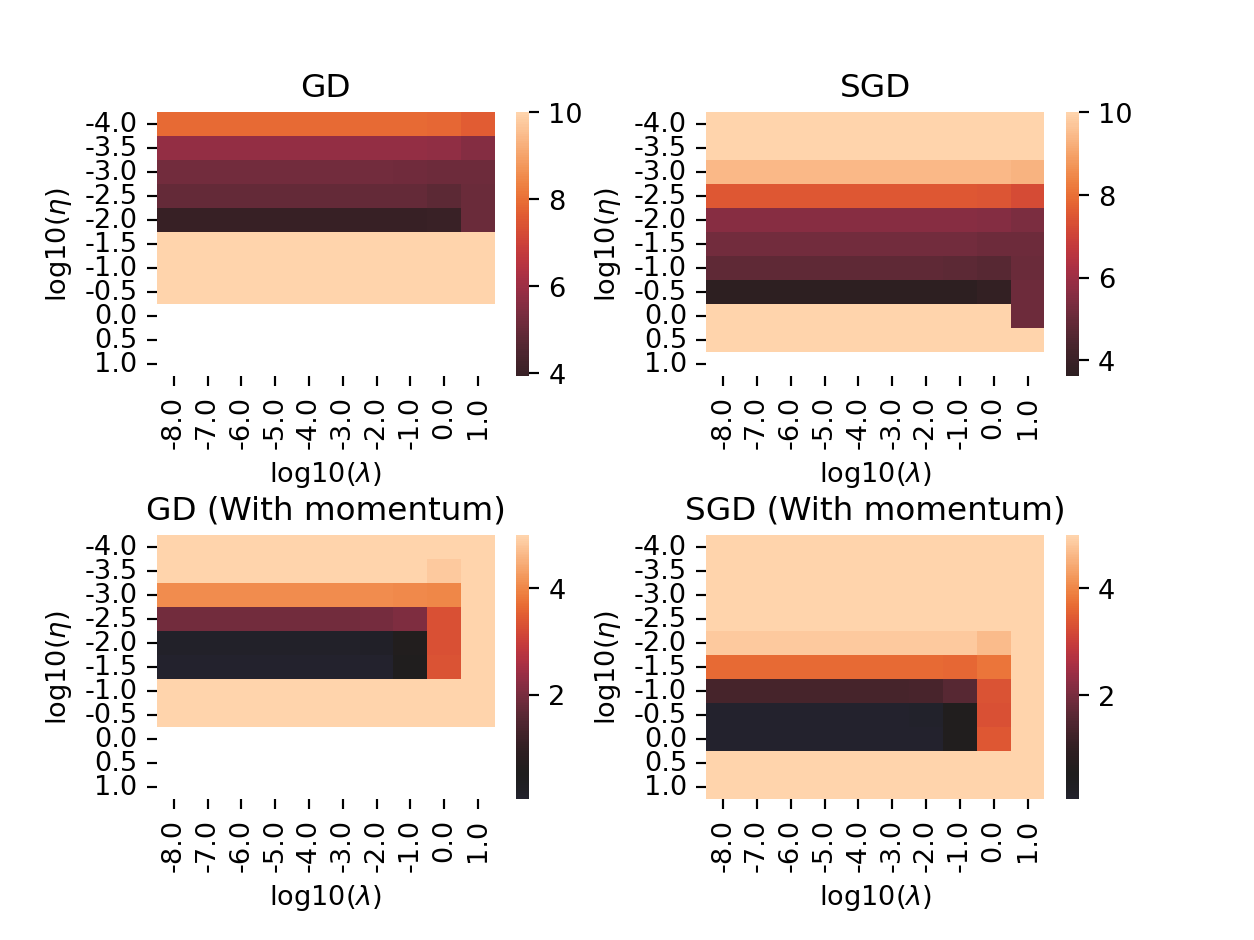
\includegraphics[scale=0.8]{optimizers_ridge_gd_sgd}
      \caption{A heatmap of the test MSEs for various learning-rates and
            regularization paramters, using GD/SGD with and without momentum. Here we
            see that the lowest test MSEs for all the methods are somewhere in the
            middle of each heatmap. We also see that too low or high of a
            learning-rate $\eta$ gives very poor or diverging costs, while too high or
            low regularization parameter $\lambda$ also gives worse performance.}
      \label{heatmapplot-lr-lambda-gd-sgd}
\end{figure}

\begin{figure}
      \centering
      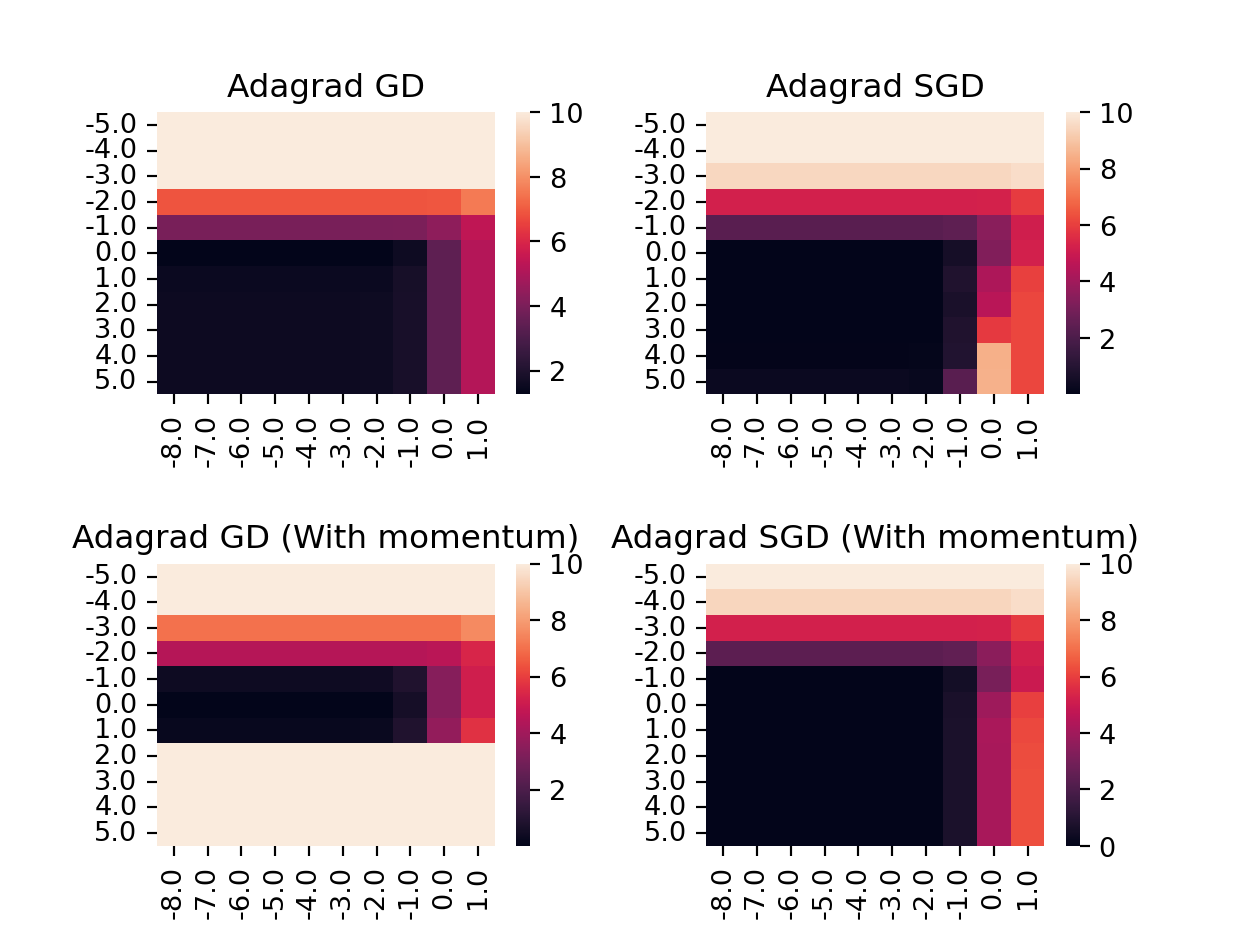
\includegraphics[scale=0.8]{optimizers_ridge_adagrad}
      \caption{A similar heatmap to \ref{heatmapplot-lr-lambda-gd-sgd}. We see
            much of the same patterns here, with one difference being that apart
            from the non-stochastic model without momentum, we are able to have
            much higher learning-rates without the costs diverging.}
      \label{heatmapplot-lr-lambda-adagrad}
\end{figure}


\subsection{The franke-function}
Experimentation of using a neural network with the franke-function is done
in the \textbf{franke\_function.py} file in the project codes
\cite{githubrepoproject2code}. We here tried to fit an neural network as good as
possible to minimize the MSE. Doing a grid-search on both the learning-rate
$\eta$ and the regularization parameter $\lambda$ for each method using only
stochastic gradient descent in this case. Figure \ref{heatmapplot-franke} shows
a heatmap of the MSE for some different values of both. Again here we see much
of the same effect as we did in figure \ref{heatmapplot-lr-lambda-gd-sgd} and
\ref{heatmapplot-lr-lambda-adagrad}, with the best performance being dependent
on having a fitting learning-rate and regularization parameter, but we can also
see that we have quite a lot of learning-rates which get get quite good results
for both train and test seemingly. Table \ref{metrics-nn-franke} shows us some
metrics we got when training neural networks on the franke-function. We get
quite good results here, and we also see that the MSE and $R^2$ scores for the
train and test-data are quite similar, which does indicate that the
regularization works quite well (though one of course need to take into account
that they were achieved at different values of $\lambda$). If we compare this to
what we got for the linear methods in project $1$ we had that for linear
regression, ridge and lasso we had test MSEs of $0.0189$, $0.0173$ and $0.0165$
respectively, with the corresponding $R^2$ scores being $0.8050$, $0.8210$ and
$0.8303$ \cite[s.~4.1]{reportproject1}. We clearly see that we have indeed
achieved better performance in this case than the simple linear models we
tackled in project 1.

We also compared our own results to those of ScikitLearn and tensorflow. Figure
\ref{metrics-nn-franke-sklearn-tf} shows the MSE achieved using these two
methods as well (here I have dropped the $R^2$ scores, but they will be closely
related to the MSEs).  Interestingly we got quite a bit better results for our
own code than these two libraries, however we have spent less time tweaking these
models and their hyperparameters, so this is probably the reason for the worse
performance here.

\begin{figure}
      \centering
      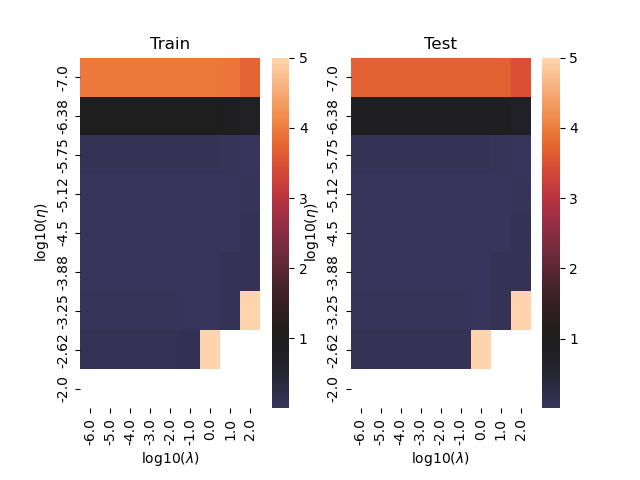
\includegraphics[scale=0.8]{heatmap_frankefunction}
      \caption{A heatmap showing the cost (MSE) for both train and test-data,
            depending the the learning-rates $\eta$ and regularization parameters
            $\lambda$.}
      \label{heatmapplot-franke}
\end{figure}

\begin{table}
      \centering
      \begin{tabular}{| c | c | c |}
                         & Train  & Test   \\
            MSE (best)   & 0.0068 & 0.0072 \\
            $R^2$ (best) & 0.9244 & 0.9266
      \end{tabular}
      \caption{The final metrics achieved using the. Here the best learning-rate
            giving best train MSE/$R^2$ score were $0.0001$, while for test MSE/$R^2$
            score the best learning-rate was $0.001$}
      \label{metrics-nn-franke}
\end{table}

\begin{table}
      \centering
      \begin{tabular}{| c | c | c |}
                        & sklearn & tensorflow \\
            MSE (train) & 0.0984  & 0.0726     \\
            MSE (test)  & 0.1091  & 0.0800
      \end{tabular}
      \caption{The MSEs when using SGD neural networks in sklearn/tensorflow,
            and using the same optimal parameters we got for our own neural net
            (though we had to use a different regularization for tensorflow). We see
            we got a little better performance using tensorflow, but still much worse
            than our own implementation (see table \ref{metrics-nn-franke})}
      \label{metrics-nn-franke-sklearn-tf}
\end{table}

Lastly we also explored using different activation functions for the hidden
layers. We here just used the same activation functions for all the hidden
layers, with us testing out sigmoid, relu and leaky relu. Table
\ref{franke-different-activ-funcs} shows the MSE for the different hidden
layers. From this we can see that the sigmoid gave us the best performance by a
little bit, so it was correct using this in our experiments above.

\begin{table}
      \centering
      \begin{tabular}{| c | c | c | c |}
                       & sigmoid & relu   & lrelu  \\
            MSE (test) & 0.0086  & 0.0178 & 0.0164
      \end{tabular}
      \caption{The test MSEs for three different activation functions. We see
            that sigmoid in particular gave about twice as low MSE as the two others,
            while relu and lrelu gave comparable results.}
      \label{franke-different-activ-funcs}
\end{table}


\subsection{Wisconsin Cancer data}
\subsubsection{Neural network}
The \textbf{neuralnet\_breastcancer.py} in the project code performs analysis for
fitting neural networks on the wisconsin breast cancer data, in a classification
task. Here we again explored various hyperparameters of the neural network to
see which hyperparameters yielded the best result. Table \ref{breastcancer-nn-hidden-layers}
shows us the accuracy and end-of-training loss for some different hidden layer sizes trained on $200$ epochs.
Here we see that all of the different layer sizes we tested were able to classify
all of the training-data correctly, so it doesn't seem to matter all that much
which of them we choose, however we do see that a model with two hidden layers,
each of $100$ nodes did give the lowest end-of-training loss so this is the
layer sizes we will be choosing for the rest of our experimentation.

\begin{table}
      \centering
      \begin{tabular}{| c | c | c | c | c | c |}
                                 & (100)    & (10, 10) & (100, 100) & (50, 10) & (10, 10, 10) \\
            Accuracy             & 1.0      & 1.0      & 1.0        & 1.0                     \\
            End of training loss & 0.001246 & 0.017191 & 0.001211   & 0.007496 & 0.014259     \\
      \end{tabular}
      \caption{Accuracy and end-of-training loss metrics for neural networks
            with different hidden layer sizes, trained using max $200$ epochs and
            using the sigmoid activation function. Here we have tested on a grid of
            learning-rates and picked the best accuracy/end-of-training loss. We see
            that all of the models are able to classify $100\%$ of the training-data
            correctly, but we see that the loss (cross-entropy) is a little lower for
            some models than others. A lower end-of-training loss indicates that the
            model learns quicker.}
      \label{breastcancer-nn-hidden-layers}
\end{table}

It is also natural to explore which activation function we shall use for the
hidden layers. Table \ref{breastcancer-nn-activ-funcs} shows the accuracy and
end-of-training loss using the three activation functions we explore in this
project. We see that all the methods perform quite well on the training-data
(when looking at the accuracy), but that the sigmoid gives a much lower
end-of-training loss, so we have much quicker learning in this case. Therefore
we choose to use the sigmoid forwards.

\begin{table}
      \centering
      \begin{tabular}{| c | c | c | c |}
                                 & sigmoid & relu     & leaky relu \\
            Accuracy             & 1.0     & 0.9774   & 0.9724     \\
            End of training loss & 0.0012  & 207.2327 & 253.2846   \\
      \end{tabular}
      \caption{The accuracy and end-of-training loss (both on the training-data)
            for a neural network with $2$ hidden layers, each with $100$ nodes and
            training on $200$ epochs. We see that overall the sigmoid does give the
            best results.}
      \label{breastcancer-nn-activ-funcs}
\end{table}
\begin{table}
      \centering
      \begin{tabular}{| c | c | c | c |}
                                 & sigmoid & relu     & leaky relu \\
            Accuracy             & 1.0     & 0.9774   & 0.9724     \\
            End of training loss & 0.0012  & 207.2327 & 253.2846   \\
      \end{tabular}
      \caption{The accuracy and end-of-training loss (both on the training-data)
            for a neural network with $2$ hidden layers, each with $100$ nodes and
            training on $200$ epochs. We see that overall the sigmoid does give the
            best results.}
      \label{breastcancer-nn-activ-funcs}
\end{table}

With the hidden layer sizes and the activation function in check we just need to
choose the learning-rate scheduler, along with the learning-rates and
regularization parameters for each of these schedulers. Table
\ref{breastcancer-nn-lr-schedulers} shows the performance of different
learning-rate schedulers in terms of prediction accuracy on both the
training-data and validation data (both for the best respective $\eta$ and
$\lambda$). Here we see that all of the models managed to give $100\%$ accuracy
on the training-data, but none of them managed it on the validation data. We see
that AdaGrad gave us the best results in this case, with the best learning-rate
being $10^{-1}$ and the best regularization parameter being $10^{-7}$. This will
then be our final chosen model.

\begin{table}
      \centering
      \begin{tabular}{| c | c | c | c | c |}
            Method              & SGD    & AdaGrad & Adam   & RMSProp \\
            Train-accuracy      & 1.0    & 1.0     & 1.0    & 1.0     \\
            Valdiation-accuracy & 0.9510 & 0.9608  & 0.9510 & 0.9510  \\
      \end{tabular}
      \caption{Training and validation accuracy. We see that AdaGrad gave
            slightly better results (one more correct prediction) than the other on
            the validation-data, while for the training-data all the schedulers are
            perfect.}
      \label{breastcancer-nn-lr-schedulers}
\end{table}

Table \ref{breastcancer-nn-final-results} shows the final accuracy evaluated on
a seperate test-set in order to not get too optimistic final metrics (we have
trained a lot of models). We here have fitted on both the previous training and
validation data. What we see is that our own neural network is able to classify
$100\%$ of the observations correctly, while the tensorflow model is able to
classify $98.55\%$ of the observations correctly. Both of these are very good
results. Figure \ref{confusion-nn-final} and \ref{confusion-nn-tf} shows the
confusion matrices for these two predictions. We see unsuprisingly that the
confusion matrix for our own neural network is perfect, while the tensorflow
version did make one wrong prediction, with it getting one false
negative.

\begin{table}
      \centering
      \begin{tabular}{| c | c | c | c | c |}
            Model         & Project NN AdaGrad & Tensorflow AdaGrad \\
            Test-accuracy & 1.0                & 0.9855             \\
      \end{tabular}
      \caption{The final accuracy on the test-data for our own custom neural
            network built from scratch, and an equivalent model fitted in tensorflow.
            Both these models use the optimal $\eta$ and $\lambda$ found previously.
            We see that we get perfect, while almost perfect performance for the
            tensorflow model.}
      \label{breastcancer-nn-final-results}
\end{table}


\begin{figure}
      \centering
      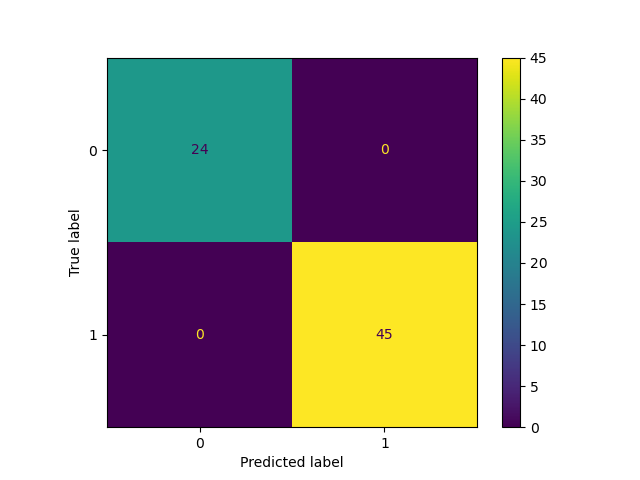
\includegraphics[scale=0.8]{confusion_matrix_nn}
      \caption{Confusion matrix for our own final AdaGrad model. We see that all the
            predictions are correctly classified.}
      \label{confusion-nn-final}
\end{figure}

\begin{figure}
      \centering
      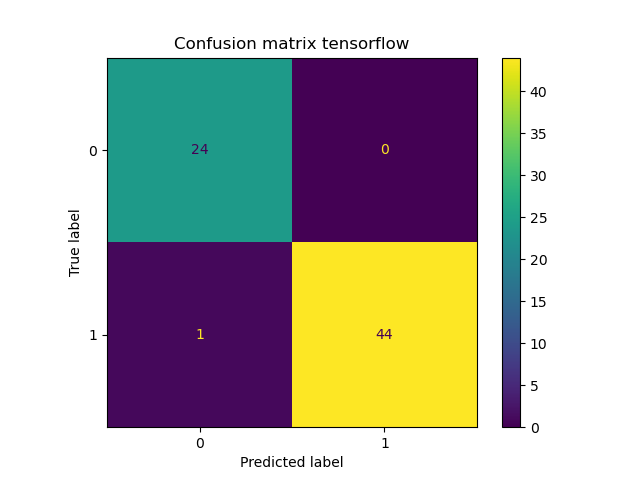
\includegraphics[scale=0.8]{confusion_matrix_tensorflow}
      \caption{Confusion matrix for the final AdaGrad model using tensorflow.}
      \label{confusion-nn-tf}
\end{figure}


\subsubsection{Logistic regression}
Finally we explored using logistic regression on the same model. Table
\ref{breastcancer-logistic-results} shows the accuracy we got on the validation
data. The results are very good with there being very few wrong predictions. We
also see that the estimated parameters for the Scikit-learn model and our own
model gave pretty much the same parameters. Lastly figure
\ref{confusion-logistic-own} shows the confusion matrix for our own logistic
regression implementation. We here see that we have one false positive and one
false negative. The confusion matrix for the sklearn-model is exactly the same.

\begin{table}
      \centering
      \begin{tabular}{| c | c | c | c | c |}
            Model         & Project Logistic & Sklearn \\
            Test-accuracy & 0.9710           & 0.9710  \\
      \end{tabular}
      \caption{The results of using logistic regression (Sklearn and own
            implementation) on the cancer data. Here we have used $\lambda = 1.0$,
            which we found out gave the best results on some validation data.
            Furthermore for both models we allowed up to $2000$ epochs and for
            the project model we used adam as the learning-rate scheduler with
            $\eta = 0.05$. We see that we get the same accuracy for our own
            model and the scikit-learn model.}
      \label{breastcancer-logistic-results}
\end{table}

\begin{figure}
      \centering
      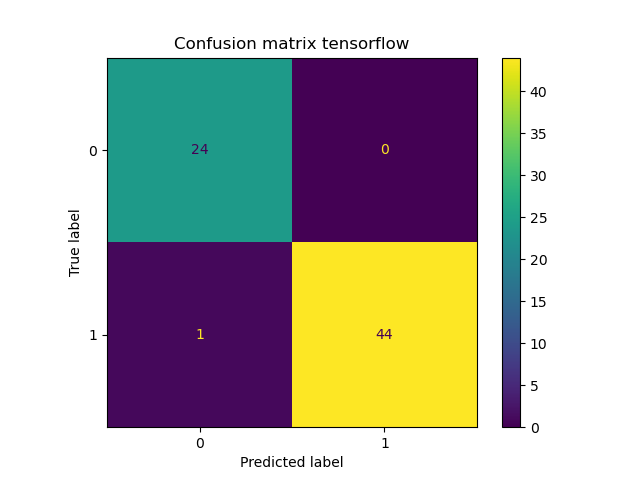
\includegraphics[scale=0.8]{confusion_matrix_tensorflow}
      \caption{Confusion matrix for the final logistic regression model (using
            our own implementation).}
      \label{confusion-logistic-own}
\end{figure}

\section{Analysis}
While exploring the hyperparameters in a neural network model that the perhaps
most central part determining how well we are able to fit the models, are the
learning-rate and regularization parameter, along with the learning-rate
scheduling method. Less important, but still noticeable is the minibatch-size,
the size and number of the hidden layers and the activation functions. This is
of course granted that the network is reasonably big enough for the task, or else
it could of course more severely impact performance (for example a very small
network wouldn't perform well on complex tasks like image-recognition). We also
clearly saw that in general the more epochs we train on the better the cost (at
least on the training-data) will generally lead to better results. We also saw
that using \textit{jax} instead of hand-computed gradients did not impact our
results.

Another thing to keep in mind is that in both the neural network for the
franke-function and for the breastcancer classification the sigmoid
activation-function gave us the best results, though in both cases relu and
leaky relu did perform not that much worse. One thing to note is that the
sigmoid activation function is more computationally heavy to use, as it involves
taking an exponential, whereas relu and leaky relu just involve a conditional
expression, each of which only contain a simple multiplication. This means that
in general training models with the sigmoid will be more computationally
expensive than the relu/lrelu versions. This way one would have to weight up if
we then could train more epochs in the same time. Here we have not done this as
we have just kept the amount of epochs the same for all these activation
functions. If we then could train more epochs in the same time on a relu/lrelu
this could very well become a better model.

We also see that the neural network we built did manage to outperform all the
linear models which we explored in project 1 (with the same amount of
observations in the train/test-data). This is likely due to the fact that in
project $1$ we mainly concentrated on fitting polynomial features up to order
$5$ and using this for our model, however seeing as our actual data is not
generated from a polynomial, but the franke-function we

Another thing to notice is that we got in both cases the best results when using
the sigmoid activation function for all the hidden layers. One thing

For the franke-function one possible improvement would be to add some different
regularizers, like for example seeing if we get improvement by using $l_1$
regularization instead of $l_2$ regularization. Another thing that could be
interesting to check out is to see how the amount of data here influences the
performance of this neural network.  One would expect that as we increase the
amount of data, that the neural network will eventually perform better than
ridge/lasso. It could be interesting to study what the boundary for this is.

Another possible improvement is that we have only tweaked some of the
hyperparameters of a neural network. Perhaps the most natural parameter to tweak
which we have left out is the momentum parameter, which we just kept fixed at
$0.9$, but this is a parameter which can have some influence over the learning
of the model. The different time-decays we have used has also been somewhat
limited, as we have only used it with stochastic gradient descent, and only in
this case used one quite basic time-decay. In general we have also used just
simple grid-search for hyperparameter-tuning, while one could use more advanced
techniques/libraries.

Lastly a potential problem I have already highlighted is how we have quite few
observations in the cancer data case. This meant our validation data in
particular became smaller than what we really wanted. One could perhaps try a
bigger split. An even better approach would be to simply split into a train-test
and then use cross-validation for selecting the hyperparameters and then
evaluate on the final model. The reason why I opted to not take this approach in
my case is mainly that cross-validation is much more computationally heavy, so
running the programs would take much longer, and they already take quite a bit
of time to run.

\section{Conclusion}
We see that when using gradient methods we have a lot of hyperparamters to tune,
with some clearly being more important than others for how good of a model we
are able to train. We have seen that especially important is the regularization
parameter $\lambda$ and learning-rate $\nu$ as well as the type of learning-rate
scheduler. Of course a high enough amount of epochs is also very important. Less
important, but still noticable is the minibatch-size when using some sort of
stochastic gradient descent, while the type of activation function and choice of
hidden layer sizes also fall into this category.

Training on the franke-function and wisconsin training-data we had that the
neural network did perform better in both of these cases on the final test data,
therefore manifesting how powerful these methods really can be. This is perhaps
especially impressive since neither of these datasets were particularly
data-heavy, which often such complex models as neural networks can struggle a
bit with. In the case of the franke-function the performance was so much better
that it seems like analysis on this, and perhaps also terrains or other
terrain-like functions, is better suited for something like a neural network
than the linear models we looked at in project 1. However in the logistic
regression case, the logistic regression was able to closely compete against
neural networks , with neural networks only just about coming out on top (also
keep in mind that our test-data was quite limited, so the significance of how
much better, if any better at all, is not all manifested). For this reason one
logistic regression (with some regularization) could still be a perfectly good
model, especially since logistic regression models are much easier to train, as
well as the fact that they are much better for cases of inference, which is
often relevant in the medical field.

\section{Appendix}

\subsection{Project code (github)}
All the python programs described in the report and with the full source code can be
found at:
\url{https://github.com/magnouvean/ml-physics-projects/tree/main/project2/python}

\bibliography{./sources.bib}

\end{document}